\documentclass{dialogue}

%\usepackage{bookta}sb

\begin{document}

\begin{otherlanguage}{english}
\begin{center}
{\Large\bfseries{Joint task learning for relation extraction and named entity recognition}}

\medskip

%Adis Davletov (\texttt{davletov-aa@ranepa.ru}), Denis Gordeev (\texttt{gordeev-di@ranepa.ru}), Alexey Rey (\texttt{rey-ai@ranepa.ru})
Authors

\medskip

%RANEPA, Moscow, Russia
Institution
\end{center}

In this work we present our system for RuREBus challenge held together with Dialog 2020 conference. The task consisted of 3 tracks: named entity recognition, relation extraction with provided named entity tags and end-to-end relation extraction. Our system took the first place in the named entity recognition track and the second place in the third track. For the second task we failed to submit the solution till the deadline but it was among the best systems. The systems for all tasks are based on Transformer models.

\textbf{Key words:} relation extraction, named entity recognition, transformer, bert
\end{otherlanguage}

\bigskip

\begin{otherlanguage}{russian}
\begin{center}
{\Large\bfseries{Совместное обучение моделей для извлечения отношений и именованных сущностей}}

\medskip

%Давлетов А. А. (\texttt{davletov-aa@ranepa.ru}), Гордеев Д. И. (\texttt{gordeev-di@ranepa.ru}), \\Рей А. И. (\texttt{rey-ai@ranepa.ru})
Авторы

\medskip

%РАНХиГС, Москва, Россия
Организация
\end{center}

В данной работе мы представляем нашу систему для соревнования RuREBus, проводящегося совместно с конференцией Dialog 2020. Задача состояла из 3 дорожек: распознавание именованных сущностей, классификация отношений между заранее аннотированными именованными сущностями и извлечение отношений из неаннотированного текста. Наша система заняла первое место в задаче распознавания именованных сущностей и второе место на третьей дорожке. Для второй задачи мы не успели своевременно представить решение, но оно оказалось в числе лучших систем. Системы для всех задач основаны на моделях Transformer.
\medskip

\textbf{Ключевые слова:} извлечение отношений, распознавание именованных сущностей, transformer, bert
\end{otherlanguage}

\selectlanguage{english}

\section{Introduction}
There are many ways to extract information from text. This task is often solved by extracting named entities and classifying relations between them. One of the most popular datasets for this task is TACRED \cite{tacred} where semantic relations are understood as relations between two pairs of entities.

Nowadays, state-of-the art results for this dataset are achieved by using Transformer-based models \cite{attention}. The most advanced models (according to https://paperswithcode.com/sota/relation-extraction-on-tacred) use extra training data.

The authors of Matching the Blanks: Distributional Similarity for Relation Learning \cite{BaldiniSoares2019}.

Knowledge Enhanced Contextual Word Representations

Among the systems that make use of only the provided data, the best results were achieved by Joshi et al. \cite{spanbert}.

Unfortunately, such annotated datasets are scarce for most languages besides English. Some researchers have tried to solve this problem for the Russian language. They have used unsupervised approaches based on knowledge databases such as Wikidata and online encyclopedias such as Wikipedia. Models trained this way tend to be not specialized because the original database does not contain relations from the required domain. They also tend to work only for the most popular relation types such as geographical or professional ones which are common to Wikipedia.

There are few annotated datasets for the Russian language. Among similar tasks to relation extraction there was held FactRuEval 2016 within the conference Dialog 2016. Within the competition contestants had to extract facts from news articles and to fill special slots in these facts (e.g. one of the fact types was 'Occupation' and its fields were 'POSITION', 'WHO', 'WHERE' and 'PHASE').

RuREBus competition was devoted to the problem of relation extraction and named entities recognition in a specialized business domain.

\section{Shared task overview}
The organizers of the competition have provided 188 annotated texts as the training dataset and 544 texts as the test dataset for the first and thirds tracks and <N> <N> for the second track respectively. All texts were provided by the Ministry of Economic Development of the Russian Federation. The corpus consists of various regional and strategic plan reports. There are in total 8 named entity classes and 11 semantic relation classes (see Tables \ref{tab:ner} and \ref{tab:rel}). The organizers have also provided a large unannotated dataset for language model fine-tuning. However, we did not use it. A named entity can consist of several words. All entities and relations do not span across sentences.

\begin{figure}[thb]
	\centering
	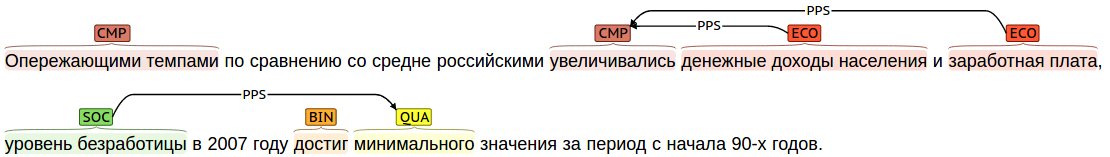
\includegraphics[scale=0.4]{pics/brat}
	\caption{RuREBus annotation example.}
	\label{fig:brat}
\end{figure}

 
Named entity groups could contain rather broad types of entities, for example "SOC" entities contained social groups as well as various social attributes - phrases like 'blue collar workers' and 'housing accessibility' corresponded to this group.

\begin{table}[bth]
	\centering
	\small
	\begin{tabular}{c||p{8cm}}
		\hline
		Type & Description\\ \hline
		MET & Some quantitative metric \\ \hline
		ECO & An economy entity or facility\\ \hline
		BIN & A binary attribute\\ \hline
		CMP & Comparative attribute\\ \hline
		QUA & Qualitative attribute\\ \hline
		ACT & Activity, actions, implemented policies\\ \hline
		INST & Institutions and organizations\\ \hline
		SOC & Social groups and characteristics\\ \hline
	\end{tabular}
	\caption{Named entity types}
	\label{tab:ner}
\end{table}
\begin{table}[bth]
	\centering
	\small
	\begin{tabular}{c|c|p{8cm}}
		\hline
		Group & Type & Description\\ \hline
		Current state of affairs & NNG & now negative \\ \hline
		Current state of affairs & NNT & now neutral \\ \hline
		Current state of affairs & NPS & now positive \\ \hline\hline

		Results & PNG & past negative\\ \hline
		Results & PNT & past neutral\\ \hline
		Results & PNS & past positive\\ \hline\hline

		Forecasts & FNG & future negative\\ \hline
		Forecasts & FNT & future neutral\\ \hline
		Forecasts & FNS & future positive\\ \hline\hline

		Goals & GOL & some abstract goals\\ \hline
		Tasks & TSK & tasks and performed actions to achieve goals\\ \hline

	\end{tabular}
	\caption{Semantic relation types}
	\label{tab:rel}
\end{table}

\section{Our solution}
The data for the competition was presented in brat format \cite{brat} where texts were given as plain txt files and annotations were provided in another file with mixed labels for named entities and relations between them. Thus, we first had to separate the labels and transform the data into special formats used by our models.

We used Razdel library to split plain texts into sentences and tokens \footnote{https://github.com/natasha/razdel}. It is a rule-based system that despite splitting sentences can also provide sentence and token offsets in the source text. Offset ranges provided by Razdel were used during preprocessing and postprocessing to map tags and relations to text spans which are required by the brat format.

After dataset tokenization we got 10460 sentences containing 336023 tokens in the train set and 20483 sentences with 643668 tokens in the test set. There are 54377 and 89006 named entity tags in the train and test sets respectively (see Table \ref{tab:tokenization}).

\begin{table}[bth]
	\centering
	\begin{tabular}{c|c|c|c|c}
		\hline
		\multicolumn{1}{c|}{Dataset} &
		\multicolumn{4}{c}{Number of} \\  \hline
		& Sentences& Tokens & NER tags & Original NER tags\\ \hline
	train & 10460 & 336023 & 54377 & 54388\\ \hline
	test & 20483 & 643668 & 89006 & 89879\\ \hline
	\end{tabular}
	\caption{Named entity types}
	\label{tab:tokenization}
\end{table}

\subsection{Named entities recognition}
The first task was to annotate named entities. First we transformed the data into the CONLL-2003 format where each line contained a word and its named entity tag. Sentences were separated with newlines. All texts were united in a single file where individual texts were divided with two empty lines. We split the data into training and validation datasets. We used a BERT-based system \cite{bert} with PyTorch model code and pretrained weights provided by Hugging Face. Due to competition being in Russian, we used the multilingual uncased base BERT model.

BERT is a Transformer based model \cite{attention}. On top of BERT outputs we added a linear layer with softmax activation function and dropout regularization. The cross entropy loss function was used to train the model. For each word token in the sentence we took BERT embedding from its first BPE-token and fed it to the dropout layer followed by the linear layer. All non entity tokens were ignored.

Our system with 0.561 micro F1-score on the public leaderboard outperformed solutions presented by other contestants.
\subsection{End-to-end relation extraction}
In subtask 3 (E2E RE) we tried the same BERT as in subtask 1 and for subtask 2 (RE with NEs) we also tried base XLM-RoBERTa model. On top of these models we are adding dropout layer followed by tag and relation linear layers. We use weighted sum of cross entropy losses for tag and relation labeling as our final loss for optimization. Padding tokens are does not contribute to our loss.
We viewed end-to-end relation extraction as a sequence labelling problem.

For end-to-end relation extraction we went with a two-stage approach. At first we used the model from the first track to label named entities. After that using the provided named entities we trained our model to predict semantic relations.

For this task we used a Roberta-based model. We viewed relation extraction as 

The data was transformed into the format used by TACRED dataset \cite{tacred}. Each relation and its corresponding entities were considered as a single training sample. We also needed to generate pairs that did not contain any relations. Thus, we randomly sampled words that had no relations between them out of sentences. The model input

<ПРИМЕР ВХОДНОГО ТЕКСТА>


The system showed 0.132 micro F1-score and it would have taken the first place among the provided systems, if we had managed to submit our solution before the deadline.

\subsection{Relation classification with provided named entity tags}
Akin to BERT-multitask learning, in this competition we wanted to experiment with simultaneous finetuning for separate tracks. RuREBus competition provided an excellent framework for this idea because we had separate tacks with different target values but the same input data.

The second and the third tracks were relation classification. In the second track the organizers provided named entity tags while in the third they did not.

For subtasks 2 and 3 we tried multitask architecture to jointly predict tags and relations. To do so, we solve relation extraction problem as sequence labeling task. In each example we have one marked entity and we are predicting relations and tags simultaneously for all tokens in the sentence. ‘0’ relation if token does not have relation to marked entity and the exact relation otherwise. To tell the system regarding which entity it should predict relations we add special tokens of the beginning and ending of the entity.


This track was very similar to end-to-end relation extraction. However, instead of using named entity labels predicted by our model, we could use the manual annotation provided by the organizers of the competition.

The model for this track is equivalent to the system used for end-to-end relation extraction. We also attempted at using the multi-task learning procedure described in previous section. However, as in the previous case the quality deteriorated when the model was trained to predict named entity tags. Thus, the loss coefficient for named entity recognition was also set to zero.
\section{Results}
All in all, our named entity recognition model with micro F1-score equal to took the first place in the competition. However, the results are lower than for other named entity recognition datasets (e.g. for the Ontonotes dataset Transformer-based models usually get > 0.85 in F1-score \footnote{see http://docs.deeppavlov.ai/en/master/features/models/ner.html}). It can be explained by the small amount of training examples and complexity of the domain.

Our end-to-end relation extraction model despite being one of the best solutions at the competition was much worse than the model trained with manual annotations provided by the organizers. 

Multi-task learning did not improve our results for this task.
\section{Conclusion}
In this work we present our system for RuREBus challenge held together with Dialog 2020 conference. The task consisted of 3 tracks: named entity recognition, relation extraction with provided named entity tags and end-to-end relation extraction. Our system took the first place in the named entity recognition track and the second place in the third track. For the second task we failed to submit the solution till the deadline but it was among the best systems. The systems for all tasks are based on Transformer models.

\section{Acknowledgments}
We would like to thank the organizers of the competition. We believe that their work will be very helpful for the development of natural language processing for the Russian language.
\bibliography{dialogue}


\end{document}
